\chapter{Analysis and Results}
\ifpdf
    \graphicspath{{Chapter3/Chapter3Figs/PNG/}{Chapter3/Chapter3Figs/PDF/}{Chapter3/Chapter3Figs/}}
\else
    \graphicspath{{Chapter3/Chapter3Figs/EPS/}{Chapter3/Chapter3Figs/}}
\fi

\section{Weight Assignment}
 
Considered here is a dataset consisting of email communications between a large network of individuals. For each email communication, information on sender(from) and receiver(to) is available. From this information, scores for edges are computed based on similarity feature and the score is associated with each edge to obtain the final weight.
Listed in the table given below are 10 of the total 59835 edges along with their corresponding weights.
  
\begin{table}[htb]
\caption{Weights for edges}
\begin{tabular}{ccl}\hline
from & to & weight\\ \hline
1 & 2 & 0.0315\\
3 & 4 & 0.0315\\
5 & 2 & 0.0315\\
6 & 7 & 0.0315\\
8 & 7 & 0.0315\\
9 & 10 & 0.0315\\
9 & 11 & 0.0315\\
12 & 13 & 0.0315\\
9 & 14 & 0.063\\
9 & 15 & 0.0315\\
\vdots&\vdots&\vdots\\ \hline
\end{tabular}\label{Table1}
\end{table}

\section{Influence Analysis}

For the network given in (\ref{Table1}) the clustering algorithm has identified 25 clusters. For each of these clusters, the scree plot is generated and the four approaches for influence analysis described in (\ref{SecIA}) are performed.
The results of this analysis for the first two clusters are shown in the figures given below.

\begin{figure}[htb]
\centering
\begin{minipage}{0.45\linewidth}
\includegraphics[scale=0.2]{Chapter3/Cluster_1_.eps}
\caption{Cluster 1}
\end{minipage}
\quad
\begin{minipage}{0.45\linewidth}
\includegraphics[scale=0.2]{Chapter3/Cluster_2_.eps}
\caption{Cluster 2}
\end{minipage}
\end{figure}
\pagebreak

\begin{figure}[htb]
\centering
\begin{minipage}{0.45\linewidth}
\includegraphics[scale=0.2]{Chapter3/Screeplot1_.eps}
\caption{Scree Plot 1}
\end{minipage}
\quad
\begin{minipage}{0.45\linewidth}
\includegraphics[scale=0.2]{Chapter3/Screeplot2_.eps}
\caption{Scree Plot 2}
\end{minipage}
\end{figure}
\pagebreak

\begin{figure}[htb]
\centering
\begin{minipage}{0.45\linewidth}
\includegraphics[scale=0.15]{Chapter3/AbsCut1_.eps}
\caption{Absolute cut score for cluster 1}
\end{minipage}
\quad
\begin{minipage}{0.45\linewidth}
\includegraphics[scale=0.15]{Chapter3/AbsCut2_.eps}
\caption{Absolute cut score for cluster 2}
\end{minipage}
\end{figure}

\begin{figure}[htb]
\centering
\begin{minipage}{0.45\linewidth}
\includegraphics[scale=0.15]{Chapter3/FixCut1_.eps}
\caption{Fixed percentage of population for cluster 1}
\end{minipage}
\quad
\begin{minipage}{0.45\linewidth}
\includegraphics[scale=0.15]{Chapter3/FixCut2_.eps}
\caption{Fixed percentage of population for cluster 2}
\end{minipage}
\end{figure}
\pagebreak

\begin{figure}[htb]
\centering
\begin{minipage}{0.45\linewidth}
\includegraphics[scale=0.15]{Chapter3/SdCut1_.eps}
\caption{Standard deviation for cluster 1}
\end{minipage}
\quad
\begin{minipage}{0.45\linewidth}
\includegraphics[scale=0.15]{Chapter3/SdCut2_.eps}
\caption{Standard deviation for cluster 2}
\end{minipage}
\end{figure}

\begin{figure}[htb]
\centering
\begin{minipage}{0.45\linewidth}
\includegraphics[scale=0.15]{Chapter3/RandomHist1_.eps}
\caption{Random Permutation Histogram for cluster 1}
\end{minipage}
\quad
\begin{minipage}{0.45\linewidth}
\includegraphics[scale=0.15]{Chapter3/RandomHist2_.eps}
\caption{Random Permutation Histogram for cluster 2}
\end{minipage}
\end{figure}
\pagebreak

\begin{figure}[htb]
\centering
\begin{minipage}{0.45\linewidth}
\includegraphics[scale=0.15]{Chapter3/RandomPlot1_.eps}
\caption{Random Permutation for cluster 1}
\end{minipage}
\quad
\begin{minipage}{0.45\linewidth}
\includegraphics[scale=0.15]{Chapter3/RandomPlot2_.eps}
\caption{Random Permutation for cluster 2}
\end{minipage}
\end{figure}

\section{Link Prediction}
 
For the network given in (\ref{Table1}) the probability of existence of an edge between any pair of nodes is computed as given in (\ref{SecLP}).
The result of this analysis is shown in the table given below.
  
\begin{table}[htb]
\caption{Probabilities for edges}
\begin{tabular}{ccl}\hline
from & to & probability\\ \hline
11 & 14 & 0.07272727\\
11 & 15 & 0.07272727\\
14 & 11 & 0.07272727\\
14 & 15 & 0.07272727\\
15 & 11 & 0.07272727\\
15 & 14 & 0.07272727\\
11 & 13 & 0.04848485\\
11 & 44 & 0.04848485\\
11 & 66 & 0.04848485\\
13 & 11 & 0.04848485\\
\vdots&\vdots&\vdots\\ \hline
\end{tabular}\label{Table2}
\end{table}

\section{Time Series Analysis}

For a social media dataset collected over time, time series analysis is performed to try and explore how this network reacts over time and how it behaves with the addition of new users, or which users tend to interact among each other. 

\begin{figure}[hb]
\centering
\begin{minipage}{0.45\linewidth}
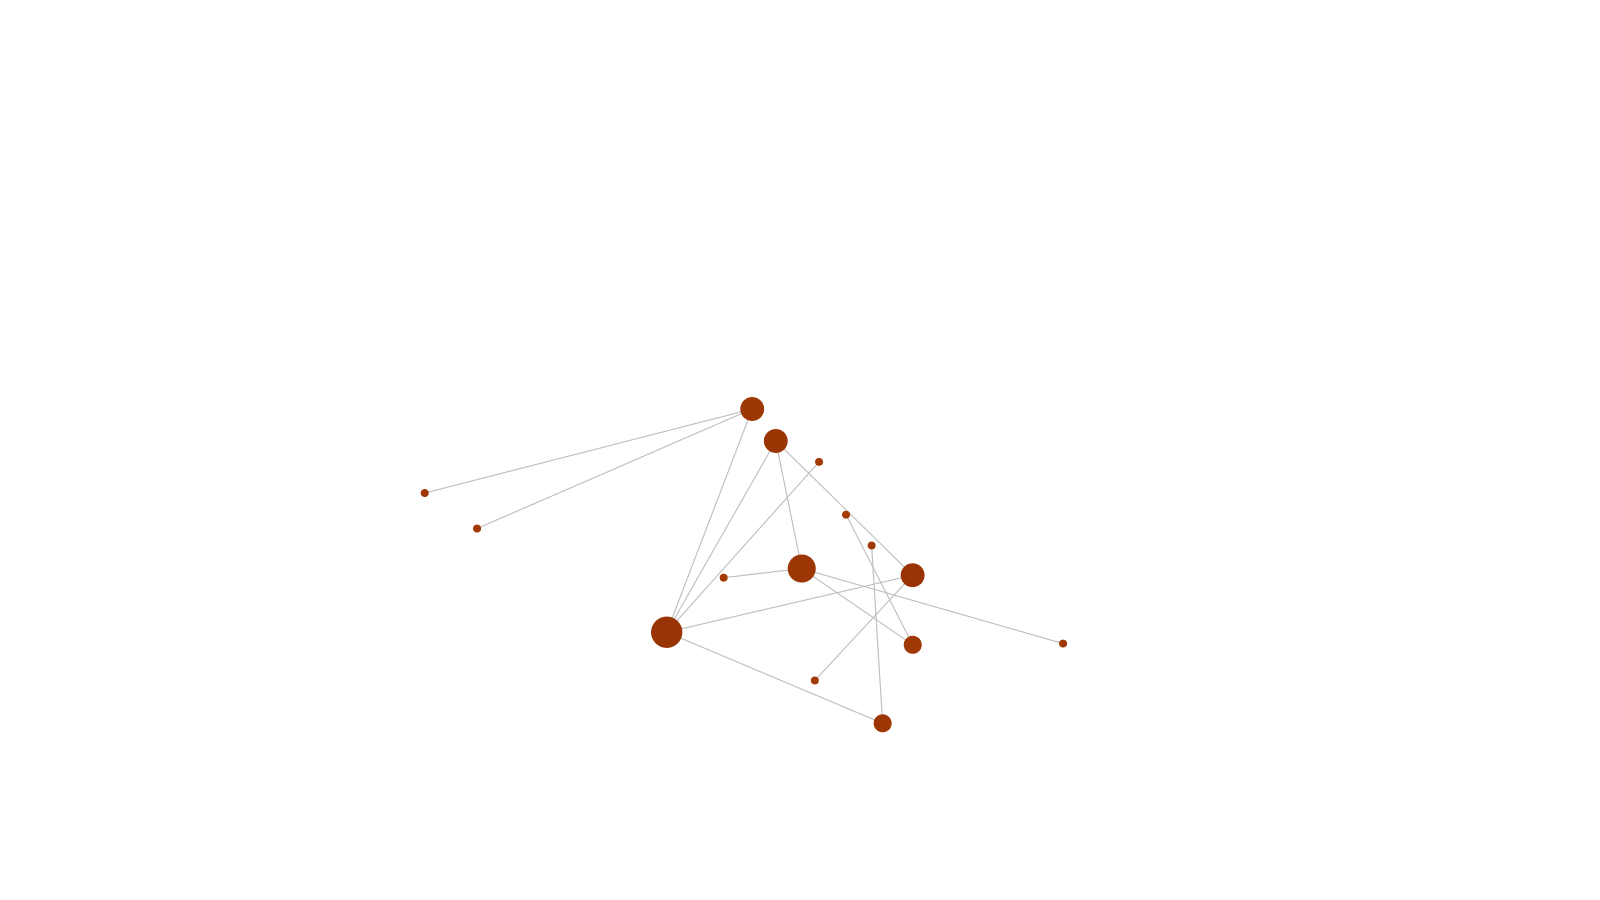
\includegraphics[scale=0.15]{Chapter3/example104.eps}
\caption{At first time instance}
\end{minipage}
\quad
\begin{minipage}{0.45\linewidth}
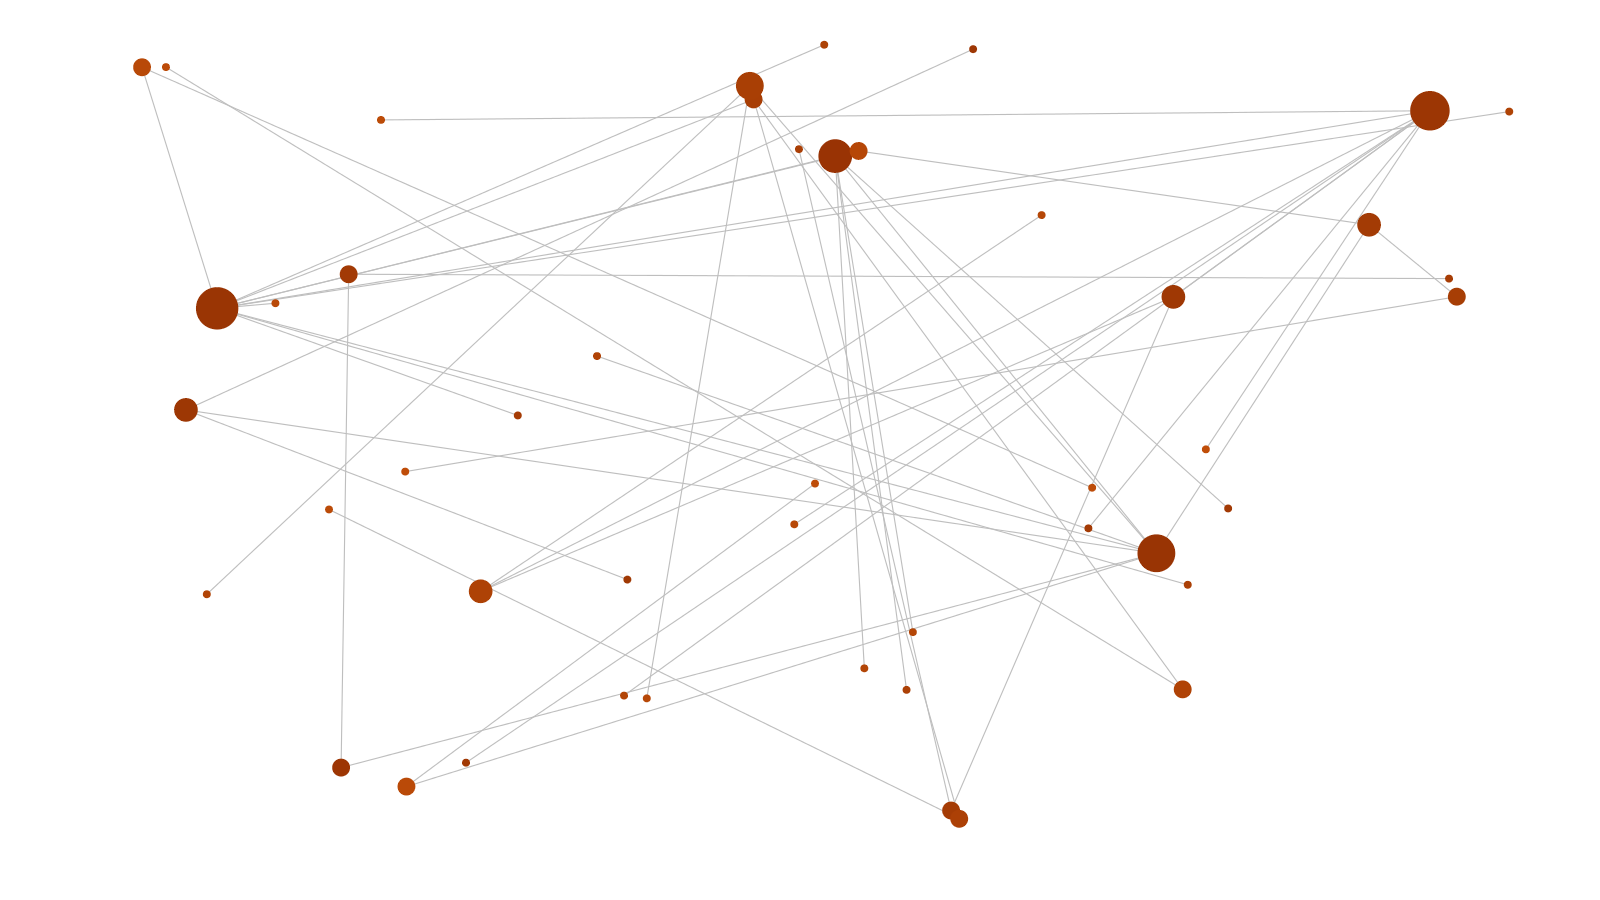
\includegraphics[scale=0.15]{Chapter3/example425.eps}
\caption{At second time instance}
\end{minipage}
\end{figure}
% ------------------------------------------------------------------------


6)  Testing, Results and Discussion

Unit testing practices have been deployed in order to test the functionality of the source code and its behaviour. We found methods in order to improve efficiency of the source code. The above problem statements were run for a variety of data-sets and thus the underlying results matched the training data-set and the testing data-sets hence establishing proof of concept. Integration testing was performed as many individual modules were integrated into a single script and was rigorously tested in order to obtain a fully functional system. Big-data paradigm was introduced and initialized to see if the concepts could function regardless of the size of the input data-set. Scalability testing was performed in order to enrich the user’s experience and to make sure that the concept could run under heavy load regardless of the input size.

Conclusion from results

We have established an agile, reliable, scalable and robust model that fulfils all the desired requirements and thus has qualified to be a fully sustainable model.

Results ( Snapshots ) (Pending)



%%% Local Variables: 
%%% mode: latex
%%% TeX-master: "../thesis"
%%% End: 
